\section{Ejericico 2}\label{sec:ejer2}


\section{Introducción}\label{sec:introduccion}
\begin{frame}{Simulación regida por tiempo}
    \textbf{Características:}
    \begin{itemize}
        \item 100 partículas posicionadas horizontalmente una al lado de la otra con resortes entre ellas.
        \item Todas las partículas cuentan con la misma masa.
        \item Solo una partícula, la número 100, se mueve sin considerar la fuerza ejercida por las otras.
        \item Las partículas tienen un movimiento principalmente vertical.
    \end{itemize}
\end{frame}

\begin{frame}{Introducción}
    \begin{block}{Diagrama:}
        \begin{figure}
            \centering
            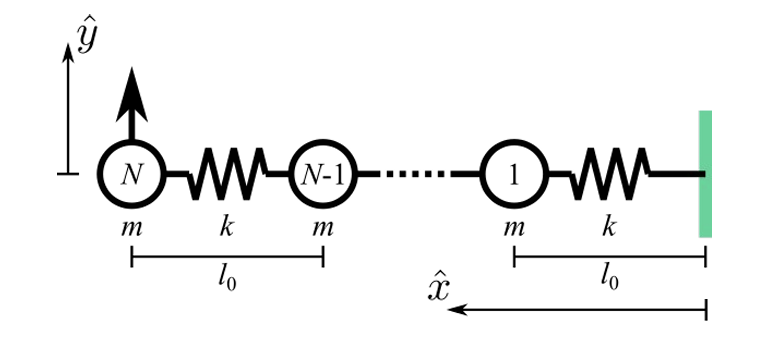
\includegraphics[width=0.8\linewidth]{pic/01-introduccion/diagrama}
        \end{figure}
    \end{block}
\end{frame}

\begin{frame}{Utilizando Verlet en los pasos temporales}
    \textbf{Fórmulas:}

    \vspace{5pt}
    \begin{equation*}
        r_i(t + \Delta{t}) = 2 r_i(t) - r_i(t-\Delta{t}) + \frac{\Delta{t}}{m_i} f_i(t) + O(\Delta{t}^4)
    \end{equation*}
    
    \vspace{20pt}
    \begin{equation*}
        v_i(t) = \frac{r_i(t+\Delta{t}) + r_i(t-\Delta{t})}{2\Delta{t}} + O(\Delta{t}^3)
    \end{equation*}
\end{frame}

\begin{frame}{Modelo}
    \begin{block}{Fuerzas Partículas 1 a 99}
        \begin{equation*}
            \begin{aligned}
                F_i(t+t_0) &= -k\ (y_i - y_{i-1}) - k\ (y_i - y_{i+1})
            \end{aligned}\label{eq:equation-particles-movement}
        \end{equation*}
        Considerando \( y_0 \) como la constante 0
    \end{block}

    \begin{block}{Partícula 100}
        Siempre seguirá el movimiento: \begin{equation*}A\ sin(\omega t)\end{equation*}
    \end{block}
\end{frame}


